
To gain deeper insight into the behavior of the Dirichlet energy during training, we conducted two additional experiments. These studies aim to clarify how energy evolves under different training dynamic, specifically in scenarios of overfitting and varying levels of label noise.


\textbf{Overfitting on clean data}

The first experiment investigates the evolution of Dirichlet energy when a model is intentionally overfitted to clean data.
We trained a GIN model on the ENZYMES dataset without regularization and with the explicit goal of fitting the training data completely. As shown in Figure~\ref{fig:enzymes_energy}, the model successfully overfits the training set, as evidenced by the near-perfect training accuracy and the large gap between training and validation accuracy.

Notably, the Dirichlet energy consistently increases throughout the training process. This finding suggests that an upward trend in energy is not necessarily caused by label noise, but may instead be a general result of overfitting. In particular, the model’s growing capacity to memorize fine-grained details may lead to less smooth and more fluctuating feature representations, reflected by higher Dirichlet energy.

\textbf{Training under varying levels of noise}

The second experiment investigates how the Dirichlet energy evolves during training when the dataset contains varying levels of label noise.
A GIN model was trained on the PPA dataset under symmetric label noise at rates of $10\%, 20\%, 30\%,$ and $40\%$. During training, we tracked the evolution of the Dirichlet energy according to the noise rate.

As illustrated in Figure~\ref{fig:noise_levels_energy}, all noise levels exhibit a similar pattern in energy evolution: an initial decrease followed by a rise. This U-shaped trajectory suggests that the model initially learns generalizable low-frequency patterns, then begins to memorize label noise, resulting in less smooth node representations and thus higher Dirichlet energy.

Crucially, we observe that higher label noise levels consistently lead to higher final Dirichlet energy. The $40\%$ noise curve ends with the highest energy, while the $10\%$ noise setting maintains the lowest. This trend highlights a direct relationship between label noise and energy growth, further suggesting that Dirichlet energy can serve as an indicator of the extent to which the model is fitting noise.





\begin{figure}[htbp]
\centering
% \setcounter{figure}{4} 

\begin{subfigure}{0.45\textwidth}
    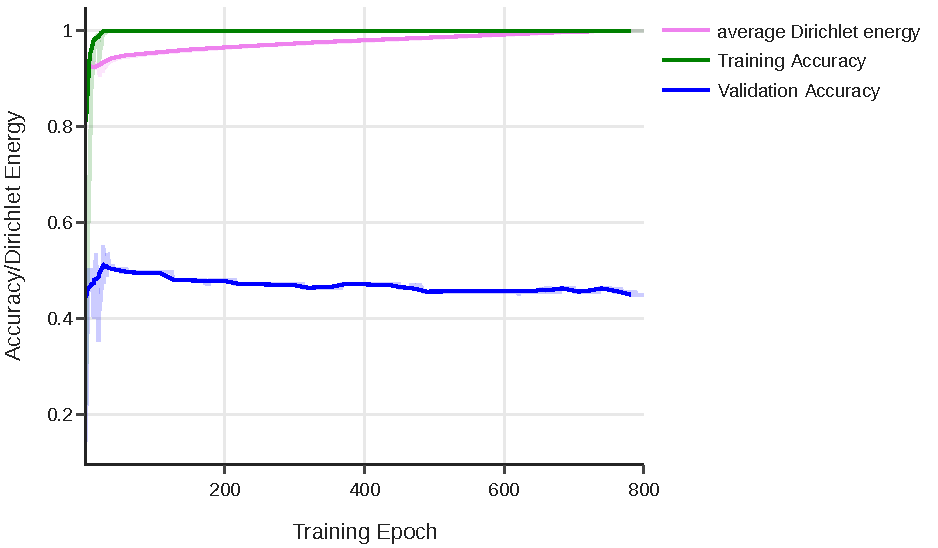
\includegraphics[width=\linewidth]{AISTATS/figures/overfit_enzyme.pdf}
    \caption{}
    \label{fig:enzymes_energy}
\end{subfigure}
\hfill
\begin{subfigure}{0.45\textwidth}
    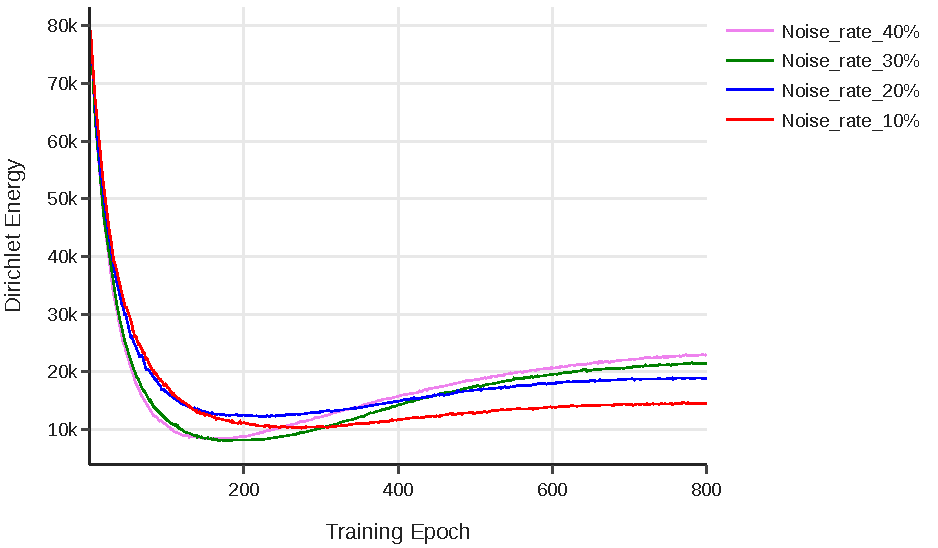
\includegraphics[width=\linewidth]{AISTATS/figures/ablation_noise.pdf}
    \caption{}
    \label{fig:noise_levels_energy}
\end{subfigure}

\caption{Empirical observations on Dirichlet energy dynamics. (a) Training on ENZYMES without noise, where the model is deliberately overfitted. The plot shows normalized Dirichlet energy alongside training and validation accuracy. As the model memorizes the training data, Dirichlet energy increases, indicating a rise in high-frequency components. (b) Evolution of normalized Dirichlet energy during training on PPA with symmetric label noise levels ($10\%$ to $40\%$). All curves follow a similar pattern: an initial energy decrease followed by a rise. Higher noise levels result in higher final energy, suggesting a link between Dirichlet energy growth and the amount of noisy labels.}
\label{fig:Additional_experiments}

\end{figure}




